\documentclass[10pt]{extarticle}
\title{}
\author{}
\date{}
\usepackage[shortlabels]{enumitem}


%paper setup
\usepackage{geometry}
\geometry{letterpaper, portrait, margin=1in}
\usepackage{fancyhdr}
% sans serif font:
\usepackage{cmbright}
%symbols
\usepackage{amsmath}
\usepackage{bigints}
\usepackage{amssymb}
\usepackage{amsthm}
\usepackage{mathtools}
\usepackage{bbm}
\usepackage[hidelinks]{hyperref}
\usepackage{gensymb}
\usepackage{multirow,array}
\usepackage{multicol}

\newtheorem*{remark}{Remark}
\usepackage[T1]{fontenc}
\usepackage[utf8]{inputenc}

%chemistry stuff
%\usepackage[version=4]{mhchem}
%\usepackage{chemfig}

%plotting
\usepackage{pgfplots}
\usepackage{tikz}
\tikzset{middleweight/.style={pos = 0.5}}
%\tikzset{weight/.style={pos = 0.5, fill = white}}
%\tikzset{lateweight/.style={pos = 0.75, fill = white}}
%\tikzset{earlyweight/.style={pos = 0.25, fill=white}}

%\usepackage{natbib}

%graphics stuff
\usepackage{graphicx}
\graphicspath{ {./images/} }
\usepackage[style=numeric, backend=biber]{biblatex} % Use the numeric style for Vancouver
\addbibresource{the_bibliography.bib}
%code stuff
%when using minted, make sure to add the -shell-escape flag
%you can use lstlisting if you don't want to use minted
%\usepackage{minted}
%\usemintedstyle{pastie}
%\newminted[javacode]{java}{frame=lines,framesep=2mm,linenos=true,fontsize=\footnotesize,tabsize=3,autogobble,}
%\newminted[cppcode]{cpp}{frame=lines,framesep=2mm,linenos=true,fontsize=\footnotesize,tabsize=3,autogobble,}

%\usepackage{listings}
%\usepackage{color}
%\definecolor{dkgreen}{rgb}{0,0.6,0}
%\definecolor{gray}{rgb}{0.5,0.5,0.5}
%\definecolor{mauve}{rgb}{0.58,0,0.82}
%
%\lstset{frame=tb,
%	language=Java,
%	aboveskip=3mm,
%	belowskip=3mm,
%	showstringspaces=false,
%	columns=flexible,
%	basicstyle={\small\ttfamily},
%	numbers=none,
%	numberstyle=\tiny\color{gray},
%	keywordstyle=\color{blue},
%	commentstyle=\color{dkgreen},
%	stringstyle=\color{mauve},
%	breaklines=true,
%	breakatwhitespace=true,
%	tabsize=3
%}
% text + color boxes
\renewcommand{\mathbf}[1]{\mathbbm{#1}}
\usepackage[most]{tcolorbox}
\tcbuselibrary{breakable}
\tcbuselibrary{skins}
\newtcolorbox{problem}[1]{colback=white,enhanced,title={\small #1},
          attach boxed title to top center=
{yshift=-\tcboxedtitleheight/2},
boxed title style={size=small,colback=black!60!white}, sharp corners, breakable}
%including PDFs
%\usepackage{pdfpages}
\setlength{\parindent}{0pt}
\usepackage{cancel}
\pagestyle{fancy}
\fancyhf{}
\rhead{Avinash Iyer}
\lhead{Algebra II: Class Notes}
\newcommand{\card}{\text{card}}
\newcommand{\ran}{\text{ran}}
\newcommand{\N}{\mathbbm{N}}
\newcommand{\Q}{\mathbbm{Q}}
\newcommand{\Z}{\mathbbm{Z}}
\newcommand{\R}{\mathbbm{R}}
\setcounter{secnumdepth}{0}
\begin{document}
  \section{Motivation and Introduction}%
  Main purpose of this course is to study Galois theory --- a field that arose in trying to study roots of polynomials.\\

  Consider $f(x) = ax^2 + bx + c$. If we want to find a general, closed-form expression for the roots of the function, we complete the square.
  \begin{align*}
    \text{roots} &= \frac{-b \pm \sqrt{b^2-4ac}}{2a}.
  \end{align*}
  We found these roots by by the coefficients, $\Q$, addition, subtraction, multiplication, division, and square root (raising to the $1/2$ power: see Math 310 notes, Page 104). Naturally, this leads us to ask whether we can do this for cubic polynomials with the same operations. Obviously, we have to change from $1/2$ power to the $1/3$ power, but Cardano showed that it was possible to solve a cubic and quartic equation using these traditional operations and radicals.\\

  Évariste Galois invented his theory to prove there is no such closed formula by radicals for any polynomial of degree $5$ or above.\\

  For example, $x^5 - x + 1$ does not have roots given by radicals.
  \subsection{Example: A Solvable Polynomial}%
  Consider the polynomial $f(x) = x^2 - 2$. We know that the roots of this polynomial are $\pm \sqrt{2}$. From this, we want to create a set $K(f)$ that satisfies the following rules:
  \begin{itemize}
    \item $\Q \subseteq K(f)$.
    \item $K(f)$ must contain the roots of $f$.
    \item $K(f)$ must be closed under the traditional operations: $+,-,\times,/$
    \item $K(f)$ must be the smallest field that satisfies the above three requirements.
  \end{itemize}
  \textbf{Claim:} $K(f) = \Q(\sqrt{2}) = \{a + b\sqrt{2}\mid a,b\in \Q\}$.
  \begin{itemize}
    \item $\Q\subseteq K(f)$, because we can set $b=0$.
    \item $\sqrt{2} = 0 + (1)(\sqrt{2})$, $-\sqrt{2} = 0 + (-1)(\sqrt{2})$
    \item Let $a+b\sqrt{2}$ and $c+d\sqrt{2}$ be elements of $K(f)$. Then,
      \begin{itemize}
        \item $(a+b\sqrt{2})\pm (c+d\sqrt{2}) = (a\pm c) + (b\pm d)\sqrt{2}$
        \item $(a+b\sqrt{2})(c+d\sqrt{2}) = (ac + 2bd) + (ad + bc)\sqrt{2}$
        \item Set $c+d\sqrt{2} \neq 0$
          \begin{align*}
            \frac{a+b\sqrt{2}}{c+d\sqrt{2}} &= \frac{(a+b\sqrt{2})(c-d\sqrt{2})}{c^2-2d^2}\\
                                            &= \frac{1}{c^2-2d^2}\left((ac-2bd) + (bc-ad)\sqrt{2}\right)\\
                                            &= \frac{ac-2bd}{c^2-2d^2} + \frac{bc-ad}{c^2-2d^2}\sqrt{2}
          \end{align*}
      \end{itemize}
    \item $K(f)$ is indeed the smallest set.
      \begin{itemize}
        \item Note that $K(f)$ is a $\Q$-vector space, with basis $\{1,\sqrt{2}\}$. Therefore, $\text{dim}_{\Q} K(f) = 2$. $K(f)$ is known as the ``splitting field'' of $f$.
      \end{itemize}
  \end{itemize}

  We want to consider a bijective function $\varphi: K(f)\rightarrow K(f)$ with the following properties:
  \begin{itemize}
    \item $\varphi(r) = r$ for every $r\in\Q$
    \item $\varphi(x+y) = \varphi(x) + \varphi(y)$
    \item $\varphi(xy) = \varphi(x)\varphi(y)$
  \end{itemize}
  We denote the collection of all such $\varphi$ as $\text{Aut}(K(f)/\Q)$. This is a group under the operation $\circ$ (composition). Specifically, we have
  \begin{align*}
    \varphi(a+b\sqrt{2}) &= \varphi(a) + \varphi(b)\varphi(\sqrt{2})\\
                         &= a + b\varphi(\sqrt{2}).
  \end{align*}
  Notice
  \begin{align*}
    \left(\varphi(\sqrt{2})\right)^2 - 2 &= \varphi \left(\left(\sqrt{2}\right)^2 - 2\right)\\
                            &= \varphi(0)\\
                            &= 0.
  \end{align*}
  Therefore, $\varphi(\sqrt{2}) = \pm \sqrt{2}$. Therefore, we have that the elements of $\text{Aut}(K(f)/\Q)$ as the following:
  \begin{align*}
    \varphi_0: a+b\sqrt{2} \mapsto a+b\sqrt{2}\\
    \varphi_1: a+b\sqrt{2} \mapsto a-b\sqrt{2}\\
    \varphi_1\circ\varphi_1 = \varphi_0\\
    \shortintertext{Thus,}
    \text{Aut}(K(f)/\Q) &= \{\varphi_0,\varphi_1\}\\
                        &\cong \Z/2\Z
  \end{align*}
  \subsection{Example: A Harder Polynomial}%
  Let $f(x) = (x^2-2)(x^2-3)$. Our roots are $\{\pm\sqrt{2},\pm\sqrt{3}\}$. We want to form $K(f)$ with the same properties. Let
  \begin{align*}
    K(f) &= \Q(\sqrt{2},\sqrt{3})\\
    &= \{a+b\sqrt{2}+c\sqrt{3}+d\sqrt{6}\mid a,b,c,d\in\Q\}.
  \end{align*}
  Just as with our previous example, $K(f)$ is a vector space over $\Q$, with basis $\{1,\sqrt{2},\sqrt{3},\sqrt{6}\}$, so $\text{dim}_{\Q}K(f) = 4$.\\

  Now, we want $\text{Aut}(K(f)/\Q)$. If $\varphi\in \text{Aut}(K(f)/\Q)$, then
  \begin{align*}
    \varphi(a+b\sqrt{2}+c\sqrt{3}+d\sqrt{6}) &= a+b\varphi(\sqrt{2}) + c\varphi(\sqrt{3}) + d\varphi(\sqrt{6})\\
                                             &= a+b\varphi(\sqrt{2}) + c\varphi(\sqrt{3}) + d\varphi(\sqrt{2})\varphi(\sqrt{3}).
  \end{align*}
  Thus, we need to know $\varphi(\sqrt{2})$ and $\varphi(\sqrt{3})$. So,
  \begin{align*}
    f(\varphi(\sqrt{2})) &= \left(\left(\varphi(\sqrt{2})\right)^2 - 2\right)\left(\left(\varphi(\sqrt{2})\right)^2-3\right)\\
                         &= 0\\
                         \shortintertext{and the same is the case with $\varphi(\sqrt{3})$. So,}
    \varphi(\sqrt{2}) &\in \{\pm\sqrt{2}, \pm\sqrt{3}\}\\
    \varphi(\sqrt{3}) &\in \{\pm\sqrt{2},\pm\sqrt{3}\}.\\
    \shortintertext{Suppose $\varphi(\sqrt{2}) = \sqrt{3}$. Then,}
    \left(\left(\varphi(\sqrt{2})\right)^2\right) &= (\sqrt{3}^2-1)\\
                                                  &= 0\\
                                                  &=\left(\varphi(2)-3\right)\\
                                                  &= -1.~\bot\\
                                                  \shortintertext{Thus,}
    \varphi(\sqrt{2}) &\in \{\pm\sqrt{2}\}\\
    \varphi(\sqrt{3}) &\in \{\pm\sqrt{3}\},\\
    \shortintertext{and we have the maps as:}
    \varphi_0&: \sqrt{2}\mapsto\sqrt{2},\sqrt{3}\mapsto\sqrt{3}\\
    \varphi_1&: \sqrt{2}\mapsto-\sqrt{2},\sqrt{3}\mapsto\sqrt{3}\\
    \varphi_2&: \sqrt{2}\mapsto\sqrt{2},\sqrt{3}\mapsto-\sqrt{3}\\
    \varphi_3&: \sqrt{2}\mapsto-\sqrt{2},\sqrt{3}\mapsto-\sqrt{3}\\
  \end{align*}
  %\begin{center}
  %  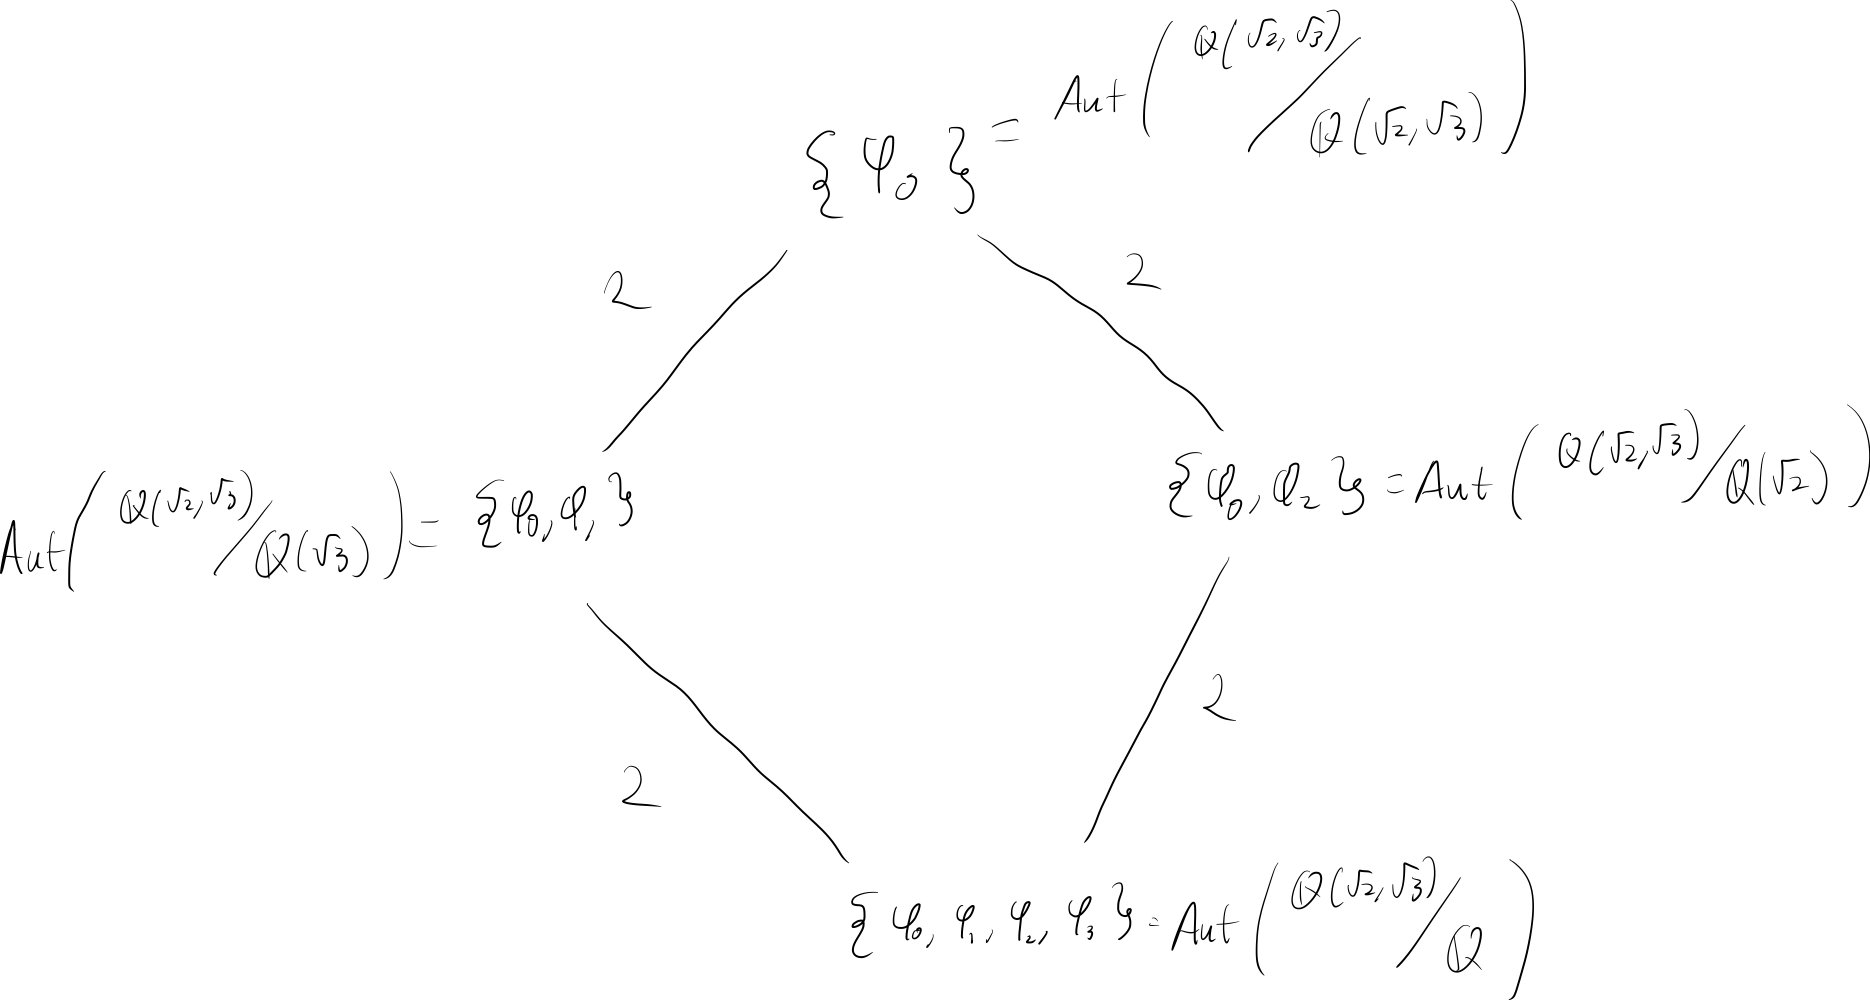
\includegraphics[width=\textwidth]{images/automorphism_lattice.png}
  %\end{center}
  % automorphism group lattice
  \section{Example: A Cubic Polynomial}%
  Consider the function $f(x) = x^3 - 2$. The function has one real root, $r_1=\sqrt[3]{2}$, and two complex roots. Let's examine $\Q(\sqrt[3]{2}) = \{a + b\sqrt[3]{2} + c\sqrt[3]{4}\mid a,b,c\in\Q\}$; $r_2$ and $r_3$ are not in $Q(\sqrt[3]{2})$. We could instead consider $\Q(\sqrt[3]{2},r_1,r_2)$.
  \begin{align*}
    x^3-2 &= (x-r_1)(x^2 + r_1x + r_1^2)\\
    r_2 &= \frac{-r_1 + \sqrt{r_1^2-4r_1^2}}{2}\\
        &= r_1\frac{-1+\sqrt{-3}}{2}\\
        &= r_1\zeta_3\\
    r_3 &= r_1\frac{-1 - \sqrt{-3}}{2}\\
        &= r_1\zeta_3^2
  \end{align*}
  However, including $r_2$ and $r_3$ is excessive --- all we need is $\Q(\sqrt[3]{2},\zeta_3)$. Therefore, the basis of this vector space is $\{1,r_1,r_1^2,\zeta_3,\zeta_3 r_1,\zeta_3 r_1^2\}$ (note that $\zeta_3^2 = -1-\zeta_3$). Therefore, $\text{dim}_{\Q}\Q(\sqrt[3]{2},\zeta_3)=6$, and $\Q(\sqrt[3]{2},\zeta_3) = K(f)$.Additionally, we have $\text{Aut}(\Q(\sqrt[3]{2})/\Q) = \{\varphi_0\}$, but $\dim_{\Q}\Q(\sqrt[3]{2}) = 3$. For the full field extension, we need to find $\varphi(\sqrt[3]{2})$ and $\varphi(\zeta_3)$.
  \begin{align*}
    \varphi(\sqrt[3]{2}) &\in \{r_1,\zeta_3 r_1,\zeta_3^2 r_1\}\\
    \varphi(\zeta) &\in \{\zeta_3,\zeta_3^2\}\\
    \varphi_0 &: r_1\mapsto r_1,\zeta_3\mapsto \zeta_3\\
    \varphi_1 &: r_1\mapsto \zeta_3r_1,\zeta_3\mapsto \zeta_3\\
    \varphi_2 &: r_1\mapsto r_1,\zeta_3\mapsto \zeta_3^2\\
    \varphi_3 &: r_1\mapsto \zeta_3^2r_1,\zeta_3\mapsto \zeta_3\\
    \varphi_4 &: r_1\mapsto \zeta_3r_1,\zeta_3\mapsto \zeta_3^2\\
    \varphi_5 &: r_1\mapsto \zeta_3^2r_1,\zeta_3\mapsto \zeta_3^2\\
    \shortintertext{Therefore,}
    \text{Aut}(\Q(\sqrt[3]{2},\zeta_3)/\Q) &= 6\\
                                           &= \dim_{\Q}\Q(\sqrt[3],\sqrt[3]{2})
  \end{align*}
\end{document}
